%%%%%%%%%%%%%%%%%%%%%%%%%%%%%%%%%%%%%%%%%%%%%%%%%%%%%%%%%%%%%%%%%%%%%%%%%%%%%%%
\section{\orangebold{Part 2.} Improving the Robustness of Convolutional Neural Networks}
%%%%%%%%%%%%%%%%%%%%%%%%%%%%%%%%%%%%%%%%%%%%%%%%%%%%%%%%%%%%%%%%%%%%%%%%%%%%%%%



% %%%%%%%%%%%%%%%%%%%%%%%%%%%%%%%%%%%%%%%%%%%%%%%%%%%%%%%%%%%%%%%%%%%%%%%%%%%%%%%
% \begin{frame}{Doubly-Block Toeplitz Matrices}
% %%%%%%%%%%%%%%%%%%%%%%%%%%%%%%%%%%%%%%%%%%%%%%%%%%%%%%%%%%%%%%%%%%%%%%%%%%%%%%%
%
%   % A block Toeplitz matrix is a matrix which contains \textbf{blocks that are repeated down the diagonals} of the matrix.
%   %
%   % A \textbf{doubly-block Toeplitz matrix} is a block Toeplitz matrix where all blocks are also Toeplitz.
%
%   \begin{minipage}{\textwidth}
%     \centering
%     Doubly-block Toeplitz Matrices are structured matrices from the Toeplitz Family.
%     % From Toeplitz matrices, we can also define \orangebold{Doubly-block Toeplitz Matrices} which are Toeplitz matrices where all blocks are also Toeplitz.
%   \end{minipage}
%   \vspace{0.3cm}
%  
%   \begin{minipage}[t]{\textwidth}
%     \centering
%     \only<1>{
%       \fbox{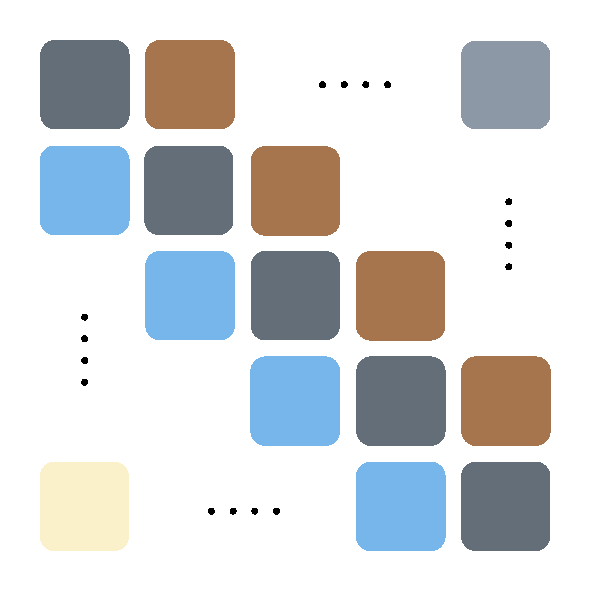
\includegraphics[scale=0.36]{images/doubly_block_v1.pdf}} \\
%       \footnotesize{Toeplitz matrices: all values are repeated down the diagonals. \\ \phantom{text}}
%     }
%     \only<2>{
%       \fbox{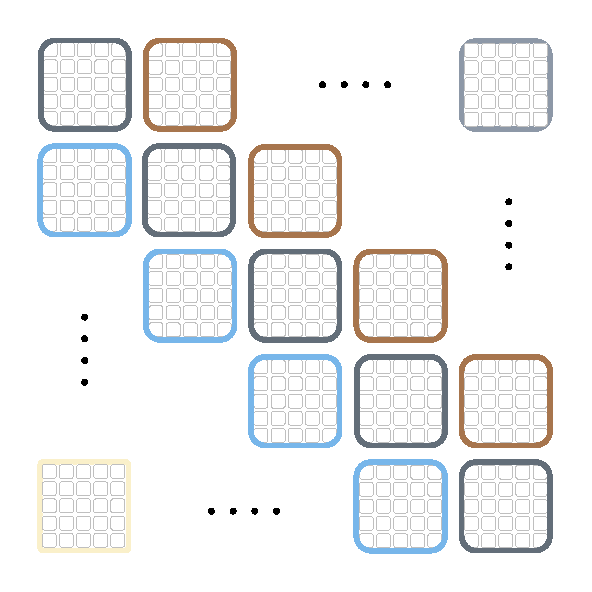
\includegraphics[scale=0.36]{images/doubly_block_v2.pdf}} \\
%       \footnotesize{Block Toeplitz matrices: all block are repeated down the diagonals. \\ \phantom{text}}
%     }
%     \only<3>{
%       \fbox{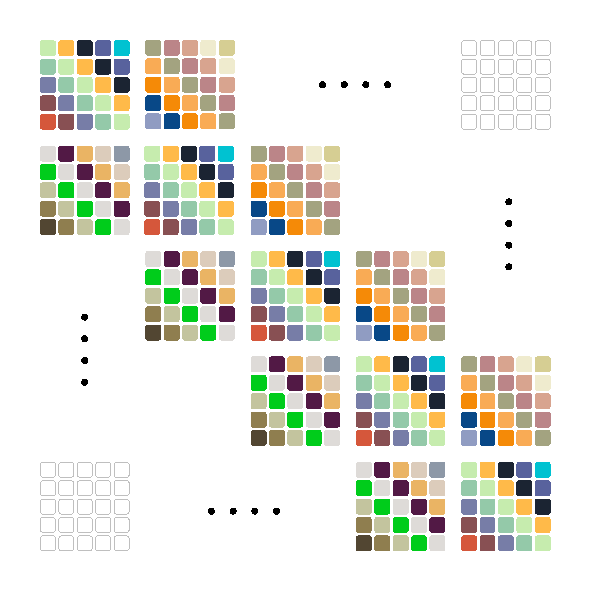
\includegraphics[scale=0.36]{images/doubly_block_v3.pdf}} \\
%       \footnotesize{Doubly-block Toeplitz matrices: each block is repeated down the diagonals \\ and the block are also Toeplitz.}
%     }
%   \end{minipage}
%
%   % \vspace{0.5cm}
%   % \visible<3>{
%   %   \begin{mdframed}[linecolor=OrangePSL,linewidth=1pt]
%   %     \centering
%   %     Doubly-block matrices are equivalent to the 2d discrete convolution.
%   %   \end{mdframed}
%   % }
%   
% \end{frame}







%%%%%%%%%%%%%%%%%%%%%%%%%%%%%%%%%%%%%%%%%%%%%%%%%%%%%%%%%%%%%%%%%%%%%%%%%%%%%%%
\begin{frame}{Defending against Adversarial Attacks}
%%%%%%%%%%%%%%%%%%%%%%%%%%%%%%%%%%%%%%%%%%%%%%%%%%%%%%%%%%%%%%%%%%%%%%%%%%%%%%%

  % with $\norm{\tau}_p \leq \epsilon$ in such a way that the Neural Network misclassifies. Therefore, an attacker aims to find the solution to the following problem:

  An \textbf{Adversarial Attack} aims to find a \orangebold{perturbation} $\tau$  such that:
  \begin{itemize}
      \visible<2->{\item[$\bullet$] the network misclassifies;}
      \visible<3->{\item[$\bullet$] $\norm{\tau}_p \leq \epsilon$ where $\epsilon$ define the ``imperceptibility'' of the perturbation.}
  \end{itemize}

  \visible<4->{
    Finding the perturbation $\tau$ can be formalize with the following problem:
    \begin{equation}
      \tau_{\Omega}^{\mathrm{adv}}(\xvec, y) \triangleq \max_{\norm{\tau}_p \leq \epsilon} L(N_\Omega(\xvec + \tau), y)
    \end{equation}
  }

  \todo{review notation}

  \visible<5->{
    One of the best empirical defense against adversarial attacks is to minimize the \orangebold{Empirical Adversarial Risk} ({\color{SkyBlue}{\cite{goodfellow2014explaining}}}): 
    \begin{equation}
      \hat{R}^{\mathrm{adv}}_m(\Omega) \triangleq \frac{1}{m} \sum_{m=1}^{m} L \left( N_\Omega(\xvec_i + \tau_{\Omega}^{\mathrm{adv}}(\xvec_i, y_i)), y_i \right)
    \end{equation}
  }


\end{frame}





%%%%%%%%%%%%%%%%%%%%%%%%%%%%%%%%%%%%%%%%%%%%%%%%%%%%%%%%%%%%%%%%%%%%%%%%%%%%%%%
\begin{frame}{Improving the robustness of Neural Networks against Adversarial Attacks}
%%%%%%%%%%%%%%%%%%%%%%%%%%%%%%%%%%%%%%%%%%%%%%%%%%%%%%%%%%%%%%%%%%%%%%%%%%%%%%%

  We can bound the adversarial risk with the empirical adversarial risk:
  \begin{equation}
    R^{\mathrm{adv}}(\Hcal) \quad \leq \quad \hat{R}^{\mathrm{adv}}_m(\Hcal) \quad +  \quad \underbrace{P^{\mathrm{adv}}(\Omega)}_{\text{Complexity}\atop\text{Penalty}}
  \end{equation}

  \vspace{-0.4cm}
  \visible<2->{
    The \orangebold{Adversarial Complexity Penalty} depends on the Lipschitz constant of the network ({\color{SkyBlue}{\citet{farnia2018generalizable}}}).
  }

  \vspace{0.2cm}
  \visible<3->{
    \begin{mdframed}[linecolor=OrangePSL,linewidth=1pt]
      \centering
      Reducing the Lipschitz constant of the Neural Network improves the robustness against adversarial attacks.
    \end{mdframed}
  }

  \visible<4->{
    \begin{minipage}{\textwidth}
      \centering
      \begin{tikzpicture}[overlay]
	\visible<5>{
          \draw[color=OrangePSL, thick] (4.9,-1.0) -- (2.2,-1.0) -- (2.2,-2.2) -- (4.9,-2.2) -- (4.9,-1.0);
          \draw (3.5, -2.5) node {\orangebold{NP-Hard Computation}};
         }
      \end{tikzpicture}
    \end{minipage}
    Combining Adversarial Training and Lipschitz regularization: 
    \begin{equation}
      \argmin_{\Omega} \frac{1}{m} \sum_{i = 1}^{m} \underbrace{\vphantom{\frac{1}{1}} L\left( N_\Omega (\xvec_i + \tau_{\Omega}^{\mathrm{adv}}(\xvec_i, y_i)), y_i \right)}_{\text{Adversarial Training}} \quad + \quad \underbrace{ \vphantom{\frac{1}{1}} \lambda \lip(N_\Omega)}_{\text{Lipschitz Regulzarization}}
    \end{equation}
  }
  
\end{frame}



%%%%%%%%%%%%%%%%%%%%%%%%%%%%%%%%%%%%%%%%%%%%%%%%%%%%%%%%%%%%%%%%%%%%%%%%%%%%%%%
\begin{frame}{Bounding the Lipschitz constant of a Neural Network}
%%%%%%%%%%%%%%%%%%%%%%%%%%%%%%%%%%%%%%%%%%%%%%%%%%%%%%%%%%%%%%%%%%%%%%%%%%%%%%%

  The Lipschitz constant of the composition of multiple functions can be upper bounded by the product of the Lipschitz constant of each function.

  \visible<2->{
    Trivial bound for neural networks:
    \begin{equation}
      \lip(N_\Omega) \leq \prod_{i=1}^p \lip(\phi^{(i)}) = \prod_{i=1}^p \sigma_1(\Wmat^{(i)})
    \end{equation}
  }

  \visible<3->{\textbf{Remarks:}}
  \begin{itemize}
    \item[$\bullet$] <3-> This bound is very expensive to compute at each step of the training.
    \item[$\bullet$] <4-> Other tighter upper bound exist but rely on SDP ({\color{SkyBlue}{\cite{fazlyab2019efficient}}})
  \end{itemize}

  \visible<5->{
    \begin{mdframed}[linecolor=OrangePSL,linewidth=1pt]
      \centering
      \textbf{Goal}: Exploit the properties of convolutions to find a fast and accurate approximation of their largest singular values.
    \end{mdframed}
  }
 
\end{frame}




%%%%%%%%%%%%%%%%%%%%%%%%%%%%%%%%%%%%%%%%%%%%%%%%%%%%%%%%%%%%%%%%%%%%%%%%%%%%%%%
\begin{frame}{Toeplitz Matrices}
%%%%%%%%%%%%%%%%%%%%%%%%%%%%%%%%%%%%%%%%%%%%%%%%%%%%%%%%%%%%%%%%%%%%%%%%%%%%%%%

  \begin{minipage}{\textwidth}
    \centering
    A Toeplitz matrix is fully determined \orangebold{by a two-sided sequence of scalars}:  
  \end{minipage} 

  \only<1,4>{
    \begin{minipage}{\textwidth}
      \begin{equation}
	\{\  
	   \underset
	     {\vphantom{\sum_{1}{1}\xleftarrow[\text{}]{}}}
	     {\asf_{-n+1} \ ,\ \dots\ , \asf_{-1}}\ ,\  
	   \asf_{0}\ , 
	   \asf_{1}\ ,\ \dots\ , \asf_{n-1}\ 
	 \}
      \end{equation}
     \end{minipage}
  }

  \only<2>{
    \begin{minipage}{\textwidth}
      \begin{equation}
	\{\  
	   \underset
	     {\vphantom{\sum_{1}{1}}\xleftarrow[\text{First Column}]{}}
	     {\asf_{-n+1} \ ,\ \dots\ , \asf_{-1}}\ ,\  
	   \asf_{0}\ , 
	   \color{black!30}{\asf_{1}\ ,\ \dots\ , \asf_{n-1}}\ 
	 \}
      \end{equation}
     \end{minipage}
  }

  \only<3>{
    \begin{minipage}{\textwidth}
      \begin{equation}
	\{\  
           {\color{black!30}{
	   \underset
	     {\vphantom{\sum_{1}{1}}\xleftarrow[\text{First Column}]{}}
	     {\asf_{-n+1} \ ,\ \dots\ , \asf_{-1}}}}\ ,\ 
	   \asf_{0}\ , 
	   \underset
	     {\vphantom{\sum_{1}{1}}\xrightarrow[\text{First Row}]{}}
	     {\asf_{1} \ ,\ \dots\ , \asf_{n-1}}\  
	 \}
      \end{equation}
     \end{minipage}
  }

  \vspace{-0.4cm}
  \begin{minipage}{\textwidth}
    \centering
    \begin{tikzpicture}[overlay]
      \visible<2>{\draw[color=OrangePSL, thick] (-0.8,-0.2) -- (-1.8,-0.2) -- (-1.8,-3.0) -- (-0.8,-3.0) -- (-0.8,-0.2);}
      \visible<3>{\draw[color=OrangePSL, thick] (1.8,-0.2) -- (-1.8,-0.2) -- (-1.8,-0.8) -- (1.8,-0.8) -- (1.8,-0.2);}
    \end{tikzpicture}
    \begin{equation}
	\Amat = \begin{pmatrix}
	   & \asf_0      & \color<2>{black!30}{\asf_1} & \color<2>{black!30}{\cdots} & \color<2>{black!30}{\asf_{n-1}} & \\ \vspace{0.1cm}
	   & \color<3>{black!30}{\asf_{-1}}   & \color<2->{black!30}{\asf_0} & \color<2->{black!30}{\ddots} & \color<2->{black!30}{\vdots} &     \\ \vspace{0.3cm}
	   & \color<3>{black!30}{\vdots}      & \color<2->{black!30}{\ddots}  & \color<2->{black!30}{\asf_0}    & \color<2->{black!30}{\asf_1} &     \\ 
	   & \color<3>{black!30}{\asf_{-n+1}} & \color<2->{black!30}{\cdots}  & \color<2->{black!30}{\asf_{-1}} & \color<2->{black!30}{\asf_0} & 
	\end{pmatrix} \phantom{ = \Amat}
    \end{equation}
  \end{minipage}

  \vspace{0.3cm}
  \visible<4>{
    The matrix $\Amat$ can be written in matrix form with respect to the matrix indexes:
    \begin{minipage}{\textwidth}
      \centering
      \begin{equation}
	\Amat = \left( \asf_{j-i} \right)_{i,j \in \{ 0, \dots, n-1 \}}
      \end{equation}
    \end{minipage}
  }

\end{frame}







%%%%%%%%%%%%%%%%%%%%%%%%%%%%%%%%%%%%%%%%%%%%%%%%%%%%%%%%%%%%%%%%%%%%%%%%%%%%%%%
\begin{frame}{Expression of Toeplitz matrices with Fourier Analysis}
%%%%%%%%%%%%%%%%%%%%%%%%%%%%%%%%%%%%%%%%%%%%%%%%%%%%%%%%%%%%%%%%%%%%%%%%%%%%%%%

  Let us define a complex-valued function $f:[0, 2\pi] \rightarrow \Cbb$ which is the \orangebold{inverse Fourier Transform} of the sequence $\{\asf_h\}_{h \in \{-n+1, \dots, n-1\}}$:
  \begin{equation}
    f(\omega) = \sum_{h = -n+1}^{n-1} \asf_h e^{\ci h \omega} \enspace.
  \end{equation}

  \vspace{-0.2cm}
  \pause
  \noindent
  \textbf{Remark:} The function $f$ is the trigonometric polynomial of degree $n-1$. 

  \vspace{0.2cm}
  \pause
  One can recover the values of the sequence using the \orangebold{Fourier transform}:
  \begin{equation}
    \asf_h = \frac{1}{2\pi} \int_0^{2\pi} e^{-\ci h \omega} f(\omega) d\omega \enspace.
  \end{equation}

  \pause
  Therefore, we can replace this expression into the matrix notation: 
  \begin{equation}
    \Amat = \left( \frac{1}{2\pi} \int_0^{2\pi} e^{-\ci (j-i) \omega} f(\omega) d\omega \right)_{i, j \in \{0, \dots, n-1\}} \enspace.
  \end{equation}

\end{frame}



%%%%%%%%%%%%%%%%%%%%%%%%%%%%%%%%%%%%%%%%%%%%%%%%%%%%%%%%%%%%%%%%%%%%%%%%%%%%%%%
\begin{frame}{Fourier analysis for Toeplitz Martrices}
%%%%%%%%%%%%%%%%%%%%%%%%%%%%%%%%%%%%%%%%%%%%%%%%%%%%%%%%%%%%%%%%%%%%%%%%%%%%%%%

  % From there, we can define an operator $\Tmat$ mapping integrable $2\pi$-periodic functions to Toeplitz matrices:
  % \begin{equation}
  %   \Tmat(f) \triangleq\leftmat\frac{1}{2\pi}\int_{0}^{2\pi}e^{-\ci(i-j)\omega}f(\omega)\,d\omega\rightmat_{i,j \in \{0, \dots, n-1\}} \enspace.
  % \end{equation}

  % \pause
  \begin{mdframed}[linecolor=OrangePSL,linewidth=1pt]
    \centering
    Why using the Fourier transform to express Toeplitz matrices ?
  \end{mdframed}

  \pause
  \vspace{0.3cm}
  \begin{theorem}[{\color{SkyBlue}{\cite{grenander1958toeplitz}}}\xspace]
    Let $\Tmat(f)$ be a Toeplitz matrix generated by the function $f$, then:
    \begin{equation}
      \sigma_1 \left( \Tmat(f) \right) \leq \sup_{\omega \in [0, 2\pi]} |f(\omega)|
    \end{equation}
  \end{theorem}

  \todo{add examples}


\end{frame}


%%%%%%%%%%%%%%%%%%%%%%%%%%%%%%%%%%%%%%%%%%%%%%%%%%%%%%%%%%%%%%%%%%%%%%%%%%%%%%%
\begin{frame}{Equivalent Reasoning for Block Toepliz Matrices}
%%%%%%%%%%%%%%%%%%%%%%%%%%%%%%%%%%%%%%%%%%%%%%%%%%%%%%%%%%%%%%%%%%%%%%%%%%%%%%%

  The same reasoning can be applied to \orangebold{Block Toeplitz matrices}.
  
  \visible<2->{
    Let $\Bmat$ be a block Toeplitz matrices determined by a two-sided sequence of \orangebold{blocks}:
    \begin{equation}
      \{\  
	 \Bsf_{-n+1} \ ,\ \dots\ , \Bsf_{-1}\ ,\  \Bsf_{0}\ , \Bsf_{1}\ ,\ \dots\ , \Bsf_{n-1}\ 
       \}
    \end{equation}
    \noindent
    where each block is a matrix of size $m \times m$.
  }

  \vspace{0.3cm}
  \visible<3->{
    Let $g: [0, 2\pi] \rightarrow \Cbb^{m \times m}$ be a matrix-valued function and the inverse Fourier Transform of the sequence $\{ \Bsf_h \}_{\{-n+1, \dots, n-1\}}$:
    \begin{equation}
      g(\omega) = \sum_{h = -n+1}^{n-1} \Bsf_h e^{\ci h \omega} \enspace.
    \end{equation}
  }

  \vspace{-0.2cm}
  \visible<4->{
    We can use the Toeplitz operator to represent block Toeplitz matrices:
    \begin{equation}
      \Bmat = \left( \frac{1}{2\pi} \int_0^{2\pi} e^{-\ci (j-i) \omega} g(\omega) d\omega \right)_{i, j \in \{0, \dots, n-1\}}
    \end{equation}
  }


\end{frame}





%%%%%%%%%%%%%%%%%%%%%%%%%%%%%%%%%%%%%%%%%%%%%%%%%%%%%%%%%%%%%%%%%%%%%%%%%%%%%%%
\begin{frame}{Extension to Doubly-Block Toeplitz matrices}
%%%%%%%%%%%%%%%%%%%%%%%%%%%%%%%%%%%%%%%%%%%%%%%%%%%%%%%%%%%%%%%%%%%%%%%%%%%%%%%

  \begin{minipage}{\textwidth}
    We extend the reasoning to doubly-block Toeplitz matrices with \orangebold{2d trigonometric polynomials}.
  \end{minipage}

  \begin{itemize}
    \item[$\bullet$] <2-> The first dimension generates the block Toeplitz structure;
    \item[$\bullet$] <3-> The second dimension generates the Toeplitz structure of each blocks.
  \end{itemize}

  \visible<4->{
    The doubly-block Toeplitz can be written with block Toeplitz notation:
    \begin{equation}
      \Dmat(f) = \leftmat \Dmat_{{\color<5>{OrangePSL}{j-i}}}(f) \rightmat_{{\color<5>{OrangePSL}{i,j}} \in \{0, \dots, n-1\}}
    \end{equation}
  }
  
  \vspace{-0.3cm}
  \visible<6->{
    where each block $\Dmat_{j-i}$ is defined as:
    \begin{equation}
      \Dmat_{j-i}(f) = \leftmat\frac{1}{4\pi^{2}}\int_{[0,2\pi]^{2}} e^{-\ci (i-j) \omega_1} e^{-\ci {\color<7>{OrangePSL}{(k-l)}} \omega_2} f(\omega_{1},\omega_{2})\,d(\omega_{1},\omega_{2})\rightmat_{{\color<7>{OrangePSL}{k,l}} \in \{0, \dots, m-1\} } .
    \end{equation}
  }

  % Because doubly-block Toeplitz matrices are \textbf{block Toeplitz} where each block is a \textbf{Toeplitz matrix}, we can extend the reasoning with a 2 dimensional function  $f: \Rbb^2 \rightarrow \Cbb$.
  %
  % The operator $\Dmat$ which maps a function $f: \Rbb^2 \rightarrow \Cbb$ to a doubly-block Toeplitz matrix of size $nm \times nm$.

\end{frame}


%%%%%%%%%%%%%%%%%%%%%%%%%%%%%%%%%%%%%%%%%%%%%%%%%%%%%%%%%%%%%%%%%%%%%%%%%%%%%%%
\begin{frame}{Bound on the singular value of Doubly-Block Toeplitz matrices}
%%%%%%%%%%%%%%%%%%%%%%%%%%%%%%%%%%%%%%%%%%%%%%%%%%%%%%%%%%%%%%%%%%%%%%%%%%%%%%%

  % We extend the result of {\color{SkyBlue}{\cite{gray2006toeplitz}}} for Doubly-Block Toeplitz Matrices.
  
  In the same way as {\color{SkyBlue}{\cite{grenander1958toeplitz}}}, we can bound the singular values of doubly-block Toeplitz matrices with their generating function.

  \visible<2->{
    \begin{theorem}[Bound on the singular values of a Doubly-Block Toeplitz]
      Let $\Dmat (f)$ be a doubly-block Toeplitz matrix generated by the function $f$, then:
      \vspace{-0.2cm}
      \begin{equation}
	\sigma_1 \left( \Dmat(f) \right) \leq \sup_{\omega_1, \omega_2 \in [0, 2\pi]^2} |f(\omega_1,\omega_2)|
      \end{equation}
      \vspace{-0.2cm}
    \end{theorem}
  }

  \begin{itemize}
    \item[$\bullet$] <3-> Let $\Wmat$ be the doubly-block Toeplitz equivalent to a convolution kernel;
    \item[$\bullet$] <4-> Let $f$ be the generating function of $\Wmat$;
    \item[\orange{$\rightarrow$}] <5-> Then, we can upper bound the Lipschitz of the convolution:
      \begin{equation}
        \lipbound(\Wmat) \triangleq \sup_{\omega_1, \omega_2 \in [0, 2\pi]^2} |f(\omega_1,\omega_2)|
      \end{equation}
   \end{itemize}

  \vspace{-0.3cm}
  \visible<6->{
    \textbf{Remark:} We have derived a similar bound for multi-channel convolution.
  }


  % \begin{minipage}{0.3\textwidth}
  %   For a given convolution kernel
  % \end{minipage}
  % \begin{minipage}{0.3\textwidth}
  %   \orange{$\Rightarrow$} 
  %
  %
  % \begin{minipage}{\textwidth}
  %   \centering
  %   In the following, for a given convolution layer parameterized by $\Wmat$, \\ we will call this bound \color{OrangePSL}{$\lipbound(\Wmat)$}
  % \end{minipage}
  %

\end{frame}


%%%%%%%%%%%%%%%%%%%%%%%%%%%%%%%%%%%%%%%%%%%%%%%%%%%%%%%%%%%%%%%%%%%%%%%%%%%%%%%
\begin{frame}{Convolution as matrix-multiplication}
%%%%%%%%%%%%%%%%%%%%%%%%%%%%%%%%%%%%%%%%%%%%%%%%%%%%%%%%%%%%%%%%%%%%%%%%%%%%%%%
  
  \todo{xxx}

  In practice, the image has multiple \textbf{channels} (\eg RGB). We refer to the number of input channels $cin$ and the number of output channels $cout$.

  \begin{figure}
    \begin{subfigure}[t]{0.49\textwidth}
      \centering
      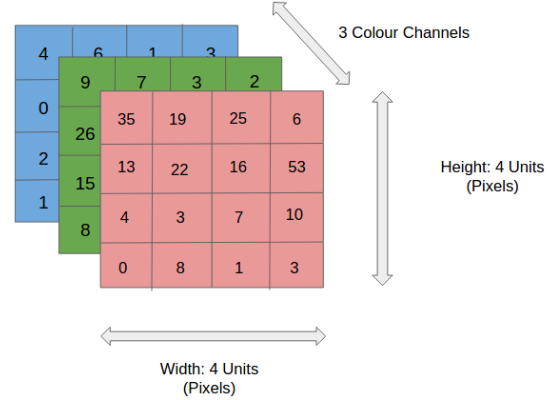
\includegraphics[width=0.8\textwidth]{images/image_rgb.png}
      \caption*{}
    \end{subfigure}
    \begin{subfigure}[t]{0.45\textwidth}
      \centering
      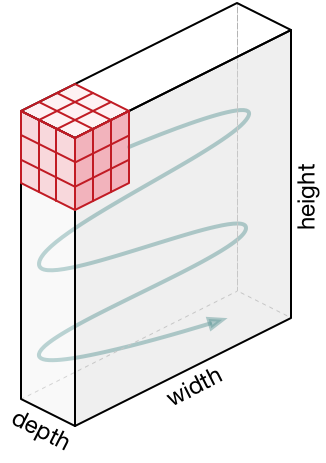
\includegraphics[width=0.5\textwidth]{images/conv_2d.png}
      \caption*{}
    \end{subfigure}
  \end{figure}

  A multi-channel convolution is equivalent to a matrix-vector product where the matrix is a \textbf{block matrix} where each block is doubly-block Toeplitz matrix. 

\end{frame}


%%%%%%%%%%%%%%%%%%%%%%%%%%%%%%%%%%%%%%%%%%%%%%%%%%%%%%%%%%%%%%%%%%%%%%%%%%%%%%%
\begin{frame}{Bound Singular Values of Convolution}
%%%%%%%%%%%%%%%%%%%%%%%%%%%%%%%%%%%%%%%%%%%%%%%%%%%%%%%%%%%%%%%%%%%%%%%%%%%%%%%

  \todo{review}

  \begin{theorem}[Bound on the maximal singular value on the convolution operation]
    Let us define doubly-block Toeplitz matrices $\Dmat(f_{11}), \dots, \Dmat(f_{\cin\times \cout})$ where $f_{ij}: \Rbb^2 \rightarrow \Cbb$ is a generating function. Construct a matrix $\Mmat$ with $\cin\times n^2$ rows and $\cout\times n^2$ columns such as
    {\small
    \begin{equation*}
	\Mmat \triangleq  \leftmat\begin{array}{ccc}
	\Dmat(f_{11}) & \cdots & \Dmat(f_{1,\cout})   \\
	\vdots & & \vdots   \\
	\Dmat(f_{\cin,1}) & \cdots & \Dmat(f_{\cin,\cout}) \\
	\end{array}\rightmat .
    \end{equation*}
    }
    Then, with $f_{ij}$ a multivariate polynomial, we have:
    \begin{equation*}
       \sigma_1(\Mmat) \leq \sqrt{ \sum_{i=1}^{\cout} \sup_{\omega_1, \omega_2 \in [0, 2\pi]^2} \sum_{j = 1}^{\cin} \left|f_{ij}(\omega_1, \omega_2) \right|^2 } .
    \end{equation*}
  \end{theorem}

  In the following, for a given convolution layer parameterized by $\Wmat$, we will call this bound $\lipbound(\Wmat)$

\end{frame}



%%%%%%%%%%%%%%%%%%%%%%%%%%%%%%%%%%%%%%%%%%%%%%%%%%%%%%%%%%%%%%%%%%%%%%%%%%%%%%%
\begin{frame}{Computing LipBound}
%%%%%%%%%%%%%%%%%%%%%%%%%%%%%%%%%%%%%%%%%%%%%%%%%%%%%%%%%%%%%%%%%%%%%%%%%%%%%%%

  \begin{minipage}{\textwidth}
    \centering
    \begin{tabular}{cccc}
      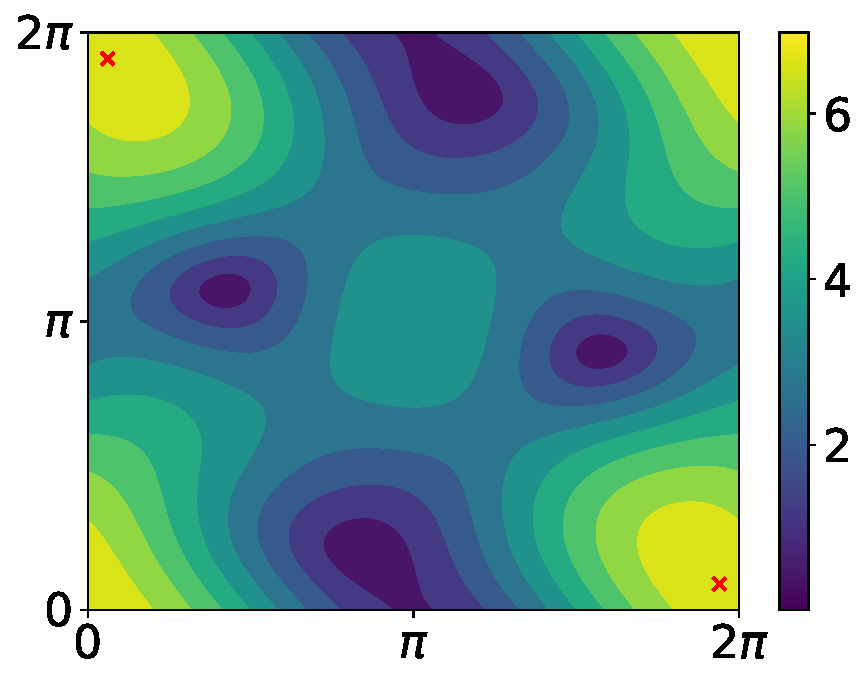
\includegraphics[scale=0.15]{images/contour_poly_200_1_1_3.pdf} &
      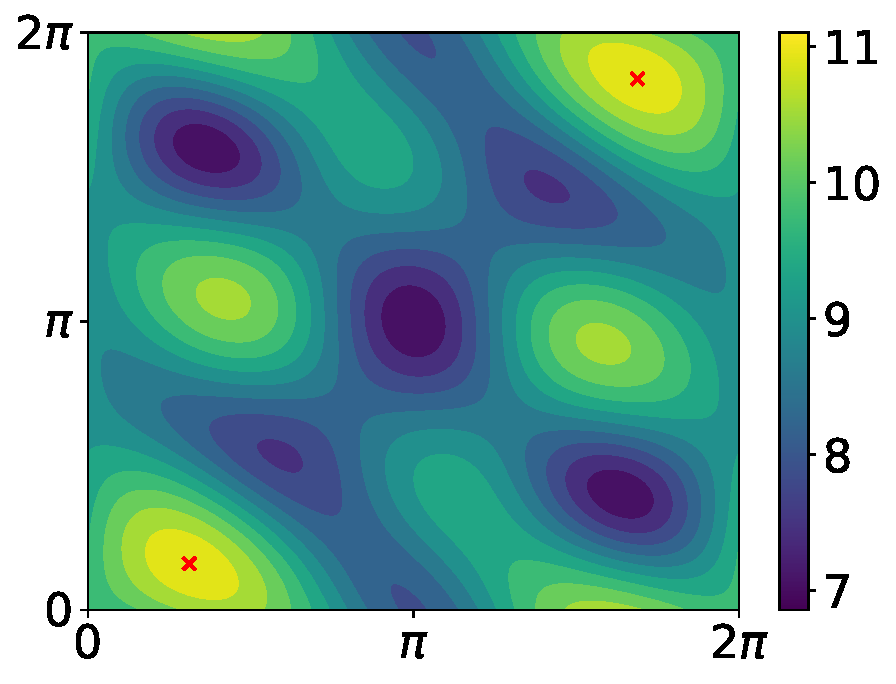
\includegraphics[scale=0.15]{images/contour_poly_200_1_9_3.pdf} & 
      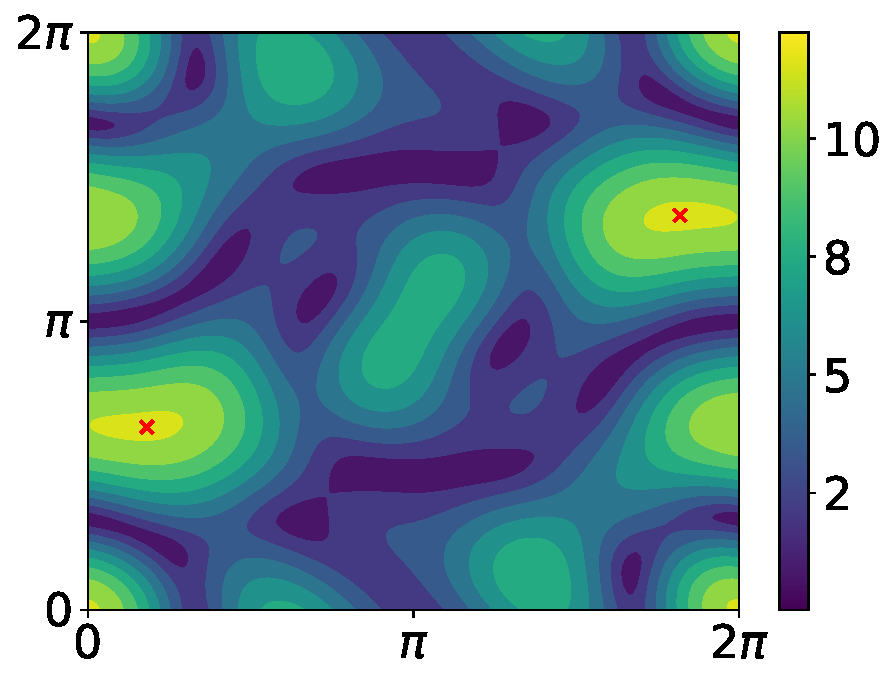
\includegraphics[scale=0.15]{images/contour_poly_200_1_1_5.pdf} & 
      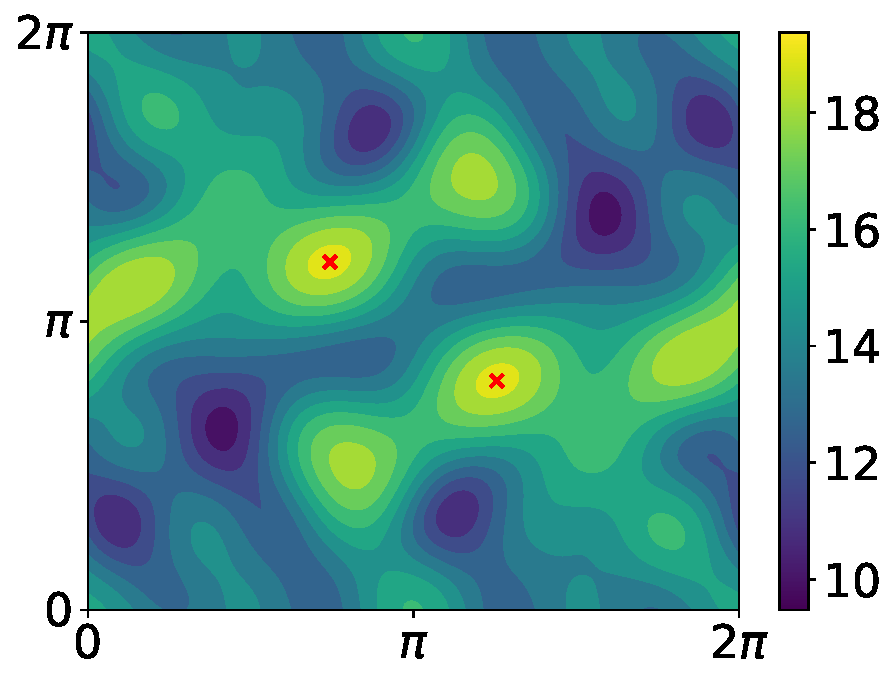
\includegraphics[scale=0.15]{images/contour_poly_200_1_9_5.pdf} \\
      \footnotesize{kernel $1\times3\times3$} &
      \footnotesize{kernel $9\times3\times3$} &
      \footnotesize{kernel $1\times5\times5$} &
      \footnotesize{kernel $9\times5\times5$}
    \end{tabular}

    \vspace{0.2cm}
    \footnotesize{Contour plot of multivariate trigonometric polynomials.}
  \end{minipage}

  \vspace{0.3cm}
  Computing $\lipbound$ implies to compute the maximum modulus of a 2-dimensional trigonometric polynomial on 
  $[ 0, 2\pi]^2$.

  \begin{itemize}
    \pause
  \item[$\bullet$] This problem has been known to be NP-hard ({\color{SkyBlue}{\cite{pfister2018bounding}}}).
    \pause
    \item[$\bullet$] However, trigonometric polynomials defined by usual convolutional kernels have a low degree (between 1 and 3)
    \pause
    \item[$\bullet$] A simple grid search algorithm is efficient and can be implemented on GPU
  \end{itemize}

\end{frame}


%%%%%%%%%%%%%%%%%%%%%%%%%%%%%%%%%%%%%%%%%%%%%%%%%%%%%%%%%%%%%%%%%%%%%%%%%%%%%%%
\begin{frame}{Precision of the Grid Search Algorithm}
%%%%%%%%%%%%%%%%%%%%%%%%%%%%%%%%%%%%%%%%%%%%%%%%%%%%%%%%%%%%%%%%%%%%%%%%%%%%%%%

  % The grid search algorithm is an approximation algorithm which takes a number of samples $S$ as input.
  % We can characterize the approximation given the number of sample used.

  \begin{itemize}
    \item[$\bullet$] We can characterize the error of the grid search algorithm with respect to the number of sample $S$.
    \visible<2->{\item[$\bullet$] Let $f: [0, 2\pi]^2 \rightarrow \Cbb$ be a two dimensional trigonometric polynomial.}
  \end{itemize}

  \vspace{0.5cm}
  \begin{minipage}{\textwidth}
    \centering
    \begin{tabular}{ccc}
      \visible<2->{
      \begin{minipage}{0.2\textwidth}
	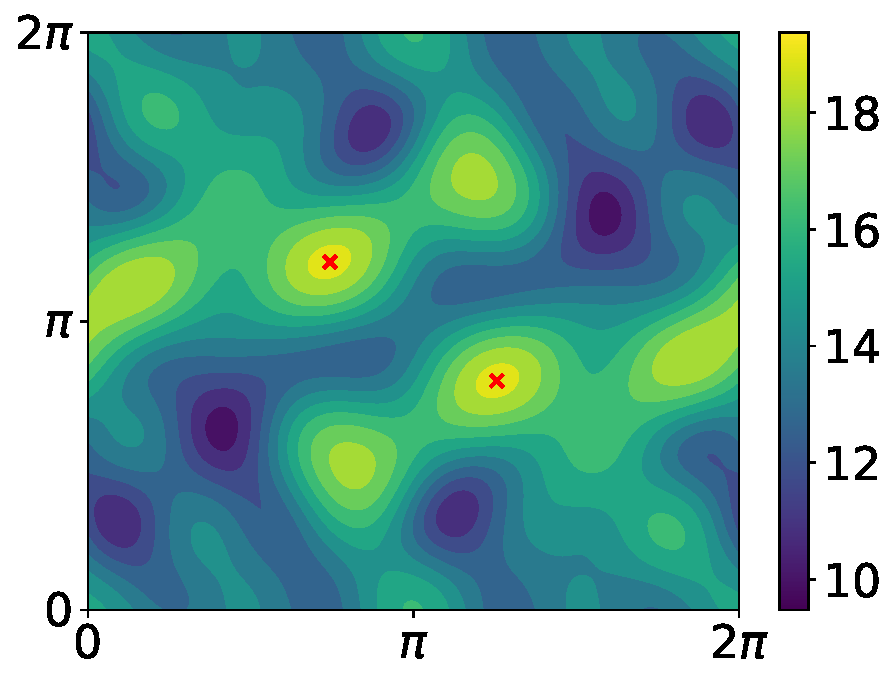
\includegraphics[scale=0.17]{images/contour_poly_200_1_9_5.pdf}
      \end{minipage}} & 
      \visible<3->{
      \begin{minipage}{0.2\textwidth}
	\centering
	$\underset{\text{discretization of}\atop\text{the search space}}{\Longrightarrow}$
      \end{minipage}} &
      \visible<3->{
      \begin{minipage}{0.2\textwidth}
	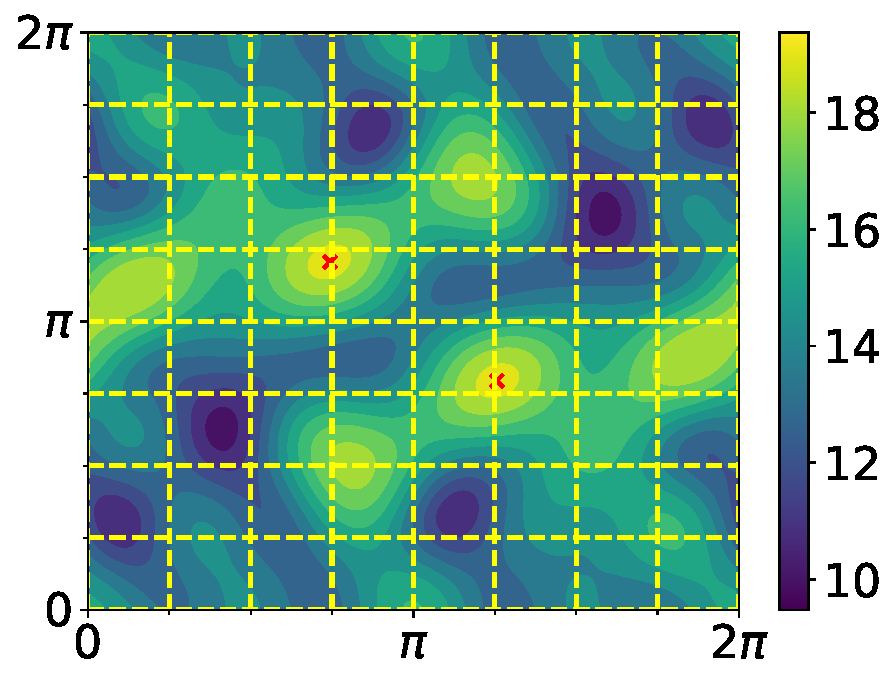
\includegraphics[scale=0.17]{images/contour_poly_200_1_9_5_grid.pdf}
      \end{minipage}} \\[1cm]
      \visible<2->{$\displaystyle \sup_{\omega_1, \omega_2 \in [0,2\pi]^2} \left| f(\omega_1, \omega_2) \right|$} & 
      \visible<4->{$\leq \left(1 - \frac{2d}{S}\right)^{-1}$} &
      \visible<3->{$\displaystyle \max_{\omega_1', \omega_2' \in \Theta_S^2} \left| f(\omega_1', \omega_2') \right|$}
    \end{tabular}
  \end{minipage}

  \vspace{0.3cm}
  \visible<4->{
    \begin{itemize}
      \item where $d$ is the degree of the polynomial.
    \end{itemize}
  }


\end{frame}



%%%%%%%%%%%%%%%%%%%%%%%%%%%%%%%%%%%%%%%%%%%%%%%%%%%%%%%%%%%%%%%%%%%%%%%%%%%%%%%
\subsection{Experiments}
%%%%%%%%%%%%%%%%%%%%%%%%%%%%%%%%%%%%%%%%%%%%%%%%%%%%%%%%%%%%%%%%%%%%%%%%%%%%%%%

%%%%%%%%%%%%%%%%%%%%%%%%%%%%%%%%%%%%%%%%%%%%%%%%%%%%%%%%%%%%%%%%%%%%%%%%%%%%%%%
\begin{frame}{Lipschitz Regularization of Convolutional Neural Networks}
%%%%%%%%%%%%%%%%%%%%%%%%%%%%%%%%%%%%%%%%%%%%%%%%%%%%%%%%%%%%%%%%%%%%%%%%%%%%%%%
 
  We want to improve upon Adversarial Training:
  % To improve the robustness of Neural Networks, we propose to minimize the following objective function:

  \begin{equation}
    \argmin_{\Omega} \frac{1}{m} \sum_{i = 1}^{m} L (N_\Omega (\xvec_i + \tau_{\Omega}^{\mathrm{adv}}(\xvec_i, y_i)), y_i) \color<1>{white}{ + \underbrace{{\color<3>{OrangePSL}{\lambda}} \sum_{j=1}^p \log(\lipbound(\Wmat^{(j)}))}_{\text{Our regularization}}}
  \end{equation}

  \visible<3->{
    where {\color<3>{OrangePSL}{$\lambda$}} is used-defined parameter which controls the regularization.
  }

  \todo{explain C\&W}
  \vspace{0.4cm}
  \visible<4->{
    $\Rightarrow$ Evaluation of the robustness: C\&W with $\ell_2$ norm ({\color{SkyBlue}{\cite{carlini2017towards}}})
  }

\end{frame}



%%%%%%%%%%%%%%%%%%%%%%%%%%%%%%%%%%%%%%%%%%%%%%%%%%%%%%%%%%%%%%%%%%%%%%%%%%%%%%%
\begin{frame}{Empirical Results}
%%%%%%%%%%%%%%%%%%%%%%%%%%%%%%%%%%%%%%%%%%%%%%%%%%%%%%%%%%%%%%%%%%%%%%%%%%%%%%%


  \begin{minipage}{\textwidth}
    \centering
    \small{
    \begin{tabular}{lc}
      \begin{tabular}{l}
	\orangebold{CIFAR10 Dataset $\quad$} \\
	50K images \\
	10 classes
      \end{tabular}
      &
      \visible<2->{
      \begin{tabular}{
	  M{l}{2-}
	  M{r}{2-}
	  M{r}{3-}
	  M{r}{4-}
	}
	\toprule
			   & \textbf{Accuracy}  & $\epsilon=0.6$ & $\epsilon = 0.8$ \\
	\midrule
        \textbf{Baseline}  & \textbf{0.95}  & 0.00          & 0.00 \\
	\textbf{AT}        & 0.86           & 0.47          & 0.33 \\
	\textbf{AT+LipReg} & 0.80           & \textbf{0.54} & \textbf{0.43} \\
	\midrule
	  &  & +0.07 & +0.10 \\
	\bottomrule
      \end{tabular}}
     \end{tabular}
     }
  \end{minipage}



  \vspace{0.8cm}
  \visible<5->{
  \begin{minipage}{\textwidth}
    \centering
    \small{
     \begin{tabular}{lc}
	\begin{tabular}{l}
	  \orangebold{ImageNet Dataset $\quad$} \\
	  1.2M images \\
	  1000 classes
	\end{tabular}
       &
       \visible<6->{
       \begin{tabular}{
	    M{l}{6-}
	    M{r}{6-}
	    M{r}{7-}
	    M{r}{8-}
          }
	 \toprule
	   & \textbf{Accuracy} & $\epsilon=1$ & $\epsilon=2$ \\
	 \midrule
	 \textbf{Baseline}  & \textbf{0.78} & 0.00          & 0.00 \\
	 \textbf{AT}        & 0.50          & 0.30          & 0.16 \\
	 \textbf{AT+LipReg} & 0.51          & \textbf{0.33} & \textbf{0.20} \\
	 \midrule
	  & & +0.03 & +0.04 \\
	 \bottomrule
       \end{tabular}}
     \end{tabular}
     }
  \end{minipage}
  }



\end{frame}











